\documentclass{article}
\usepackage[utf8]{inputenc}
\usepackage{pdfpages}
\input{Opsætning/Pakker}


\begin{document}

\begin{titlepage} % Suppresses displaying the page number on the title page and the subsequent page counts as page 1
	\newcommand{\HRule}{\rule{\linewidth}{0.5mm}} % Defines a new command for horizontal lines, change thickness here
	
	\center % Centre everything on the page
	%------------------------------------------------
	%	READ ME
	%------------------------------------------------
	   
	    %This version of the title page contains both signatures and pictures of participants, this version is best suited for larger reports and or projects. 
	
	%------------------------------------------------
	%	Headings
	%------------------------------------------------
	
	\textsc{\LARGE Danmarks Tekniske Universitet}\\[1.5cm] % Main heading such as the name of your university/college
	
    
\includegraphics[scale=0.15]{Opsætning/DTULogo.png}\\
	%\textsc{\Large Major Heading}\\[0.5cm] % Major heading such as course name
	
	%\textsc{\large Minor Heading}\\[0.5cm] % Minor heading such as course title
	
	%------------------------------------------------
	%	Title
	%------------------------------------------------
	
	\HRule\\[0.5cm]
	
	{\huge\bfseries Bachelor Projekt}\\[0.4cm] % Title of your document

	\HRule\\[0.5cm]
	%\textsc{\Large Danmarks Tekniske Universitet}\\[0.5cm] % Major heading such as course name
	
	\textsc{\Large title}\\[1cm] % Minor heading such as course title
	
	%------------------------------------------------
	%	Author(s)
	%------------------------------------------------
    \vfill\vfill\vfill
    \begin{minipage}{\textwidth}
		\begin{flushleft}
            \centering

            Jonas Dahl Larsen (s205829)
            

		\end{flushleft}
	 \end{minipage} 
    % \\[1cm]
    % \vfill \vfill
    \vspace*{1\baselineskip}


    


	%------------------------------------------------
	%	Date
	%------------------------------------------------
	
	%\vfill\vfill\vfill % Position the date 3/4 down the remaining page
	
	{\large \today} % Date, change the \today to a set date if you want to be precise
	
	\vfill % Push the date up 1/4 of the remaining page
	
\end{titlepage}
\tableofcontents
\newpage
\section{Introduktion}


I 2023 valgte Danmarks Tekniske Universitet at anvende Python som et hjælpeværktøj i deres grundlæggende matematikkursus "01001 Matematik 1a (Polyteknisk grundlag)". Python er et af de mest anvendte programmeringssprog \footnote{https://www.statista.com/statistics/793628/worldwide-developer-survey-most-used-languages/}, kun overgået af to sprog, der primært bruges sammen til at udvikle hjemmesider. Derfor har Python, med sit dynamiske skrevne sprog og en række matematiske programudvidelser som SymPy \footnote{https://www.sympy.org/en/index.html}, været et oplagt valg som programmeringssprog til det grundlæggende matematikkursus tilbudt af DTU.

Projektet vil undersøge, hvordan et funktionsprogrammeringssprog, kan gavne de studerendes forståelse af de grundlæggende matematiske koncepter. Formålet er at guide læseren gennem opbygningen af en række funktionsprogrammer baseret på grundlæggende universitetsmatematik og dermed illustrere anvendelser. Projektet beskriver en generel struktur til opbygning og anvendelse af et funktions programmeringsprogram. Der tages udgangspunkt i F\# \footnote{https://en.wikipedia.org/wiki/F\_Sharp\_(programming\_language)}, men beskrivelserne af programmerne vil også kunne anvendes i lignende funktionsprogrammeringssprog.

Rapporten begynder med at forklare nogle Fundamentale koncepter inden for funktionsprogrammering samt metoder til validering af programmerne. 


\section{Fundamentale koncepter}
\subsection{Introduktion til Funktions Programmering}
Det forventes, at læseren har kendskab til programmering. Der gives derfor kun en kort beskrivelse af syntaks og notation, så læsere, der ikke er bekendt med F\#, kan forstå de eksempler, der løbende vil forekomme i rapporten. Vi begynder derfor med at betragte funktionen for fakultet Ligning \eqref{Fakultet}.

\begin{equation}
    \label{Fakultet}
    f(n) = \begin{cases} 
            1 &  n = 0  \\
            n \cdot f(n-1) & n > 0 \\
            \text{undefined} & n < 0 
           \end{cases}
\end{equation}

Et eksempel på en implementering i F\# er givet i Listing \ref{lst:fsharp_factorial}, som kan sammenlignes med Python-koden i Listing \ref{lst:python_factorial}, da Python og pseudokode er næsten det samme.


\begin{lstlisting}[language={FSharp}, label={lst:fsharp_factorial}, caption={Eksempel på Fakultet i F\#}]
// Fakultet i F#
let rec factorial n =
    match n with
    | 0             -> 1 
    | x when x > 0  -> x * factorial (x - 1)
    | _             -> failwith "Negative argument"
\end{lstlisting}

\begin{lstlisting}[language={FSharp}, label={lst:python_factorial}, caption={Eksempel på Fakultet i Python}]
# Fakultet i Python
def factorial(n):
    if n == 0:
        return 1
    elif n > 0:
        return n * factorial(n - 1)
    else:
        raise ValueError("Negative argument")
\end{lstlisting}

I F\# anvendes \textcolor{blue}{let} til at definere en ny variabel eller, i dette tilfælde, en funktion kaldet \textcolor{red}{factorial}. Næste nøgleord er \textcolor{blue}{rec}, hvilket indikerer, at funktionen er rekursiv. Funktionen tager et inputargument \(n\), og i linje 3 starter et match-udtryk. Her er \(n\) vores udtryk, og efter \textcolor{codepurple}{with} begynder en række mønstre, som udtrykket forsøger at matche på, separeret med '\(\vert\)'. Resultatet af funktionen vil være den kode, der eksekveres efter '\(\rightarrow\)', på den linje, hvor mønsteret er genkendt.
    
I F\#, er det som udgangspunkt ikke nødvendigt at anvende parenteser som i andre programmeringssprog. Derfor vil de kun blive anvendt, hvor det er nødvendigt gennem rapporten, typisk i sammenhænge med kædning af funktioner. For at undgå brugen af parenteser kan man i F\# benytte pipe-operatorerne, $|>$ og $<|$, som fører resultatet fra en udledning direkte ind i den næste funktion. Nedenstående eksempel viser tre ækvivalente udtryk, der demonstrerer anvendelsen af disse operatorer.

\begin{lstlisting}[style=output, label={lst:pipe_operator}, caption={Eksempel på anvendelse af pipe-operatorer i F\# ved udregning af $(3!)! = 6! = 720 $.}]
> factorial (factorial 3);;
val it: int = 720

> factorial <| factorial 3;;
val it: int = 720

> factorial 3 |> factorial;;
val it: int = 720
\end{lstlisting}


% Et match på et mønster er ikke det samme som '==' kendt fra andre programmeringssprog. I linje 4 forsøger den at tildele værdien af \(n\) til 0, og dette lykkes kun, hvis \(n\) er 0. Hvis \(n\) ikke er 0 og dermed ikke genkender linje 4, vil den forsøge at genkende det næste mønster. Her står der kun \(x\), da der ikke yderligere specificeres om netop \(x\), vil det altid lykkes, og \(x\) bliver tildelt værdien af \(n\) svarende til \( [x \mapsto n] \). Derefter skal betingelserne efter \textcolor{codepurple}{when} være opfyldt. Hvis de er det, kan mønsteret genkendes på den givne linje. Derefter eksekverer den koden efter '$\rightarrow$', hvor den samtidig har adgang til den nyligt tildelte værdi af \(x\). 
% Det sidste mønster på linje 6 anvender '\textunderscore' som mønster. 
% Dette betyder, at det kan genkende alle udtryk, men vi er ikke interesseret i at anvende værdien. I dette tilfælde kan det tredje mønster på linje 6 kun køres, når \(n\) er negativ.


\subsection{Typer}
I F\#, i modsætning til Python, er typer tildelt ved kompileringstidspunktet, ikke under kørsel. Alle udtryk, inklusiv funktioner, har en defineret type. Typen for funktionen i Listing \textcolor{red}{\ref{lst:fsharp_factorial}} er $int \rightarrow int$. Det betyder, at det ikke er muligt at kalde funktionen med et argument, der ikke er af typen $int$. Typen for funktionen beskrives som $Factorial: int \rightarrow int$. Det ses dermed tydeligt hvordan f\# benytter notationen for afbildninger i mattematik, da den matematiske funktion for fakultet er en afbildning $f: \mathbb{Z} \to \mathbb{Z}$. Vi kan derfor formulere følgende omkring typer\footcitetitle[14]{HansenRischelFSharp}:
\begin{gather*}
    f: T_1 \rightarrow T_2 \\
    f(e) : T_2 \iff e : T_1
\end{gather*}
% => f(e) ville give en fejl, hvis ikke e er af typen T1
% <= per definition, så er f(e) : T2, hvis e : T1

Hvis en funktion kaldes med et argument, der ikke matcher funktionens type, genereres en fejlmeddelelse. Derudover kan en type også bestå af en tuple af typer:
\begin{gather*}
    f: T_1 * T_2 * .. * T_n \rightarrow T_{n+1}\\
    f (e_1, e_2, .., e_n) :T_{n+1} \iff e_1 : T_1 \land e_2 : T_2 \land .. \land e_n : T_n
\end{gather*}
En tuple, der kun består af to typer, kaldes et par. Givet en funktion $g: T_1 \rightarrow T_2 \rightarrow T_3$, betyder dette, at den tager et udtryk af typen $T_1$, som giver en funktion af typen $T_2 \rightarrow T_3$, hvor evalueringen af funktionen resulterer i $T_3$. Som eksempel på dette kan vi definere en multivariable funktion $f(x, y) = \sqrt{x! + y!}$ som er en afbildning $f: \mathbb{Z}^2 \to \mathbb{R}$ samt $g(y) = f(3, y) = \sqrt{3! + y!}$ som afbilder $g: \mathbb{Z} \to \mathbb{R}$, de tilsvarende F\# funktion kan defineres på følgende måder:
\begin{lstlisting}[language={FSharp}, label={lst:multivariable_function}, caption={Eksempel typerne for en multivariable funktion i F\#}]
// f: int -> int -> float
let f x y = sqrt <| float(factorial x + factorial y)

// g: int -> float
let g = f 3
\end{lstlisting}





\subsection{Signatur filer og implementerings filer}
En standard F\# fil er lavet med .fs extension, denne fil indeholder alt den kode som er nødigt for at kunne køre programmet. En implementerings fil kan have en signatur fil med .fsi extension, denne fil indeholder en beskrivelse af de typer og funktioner i implementerings filen som er tilgængelige for andre filer. En signatur fil kan derfor bruges som et blueprint for andre der ønsker at anvende eller replicere implementerings filen. I andre programmerings sprog vil man anse funktionerne i signatur filen som værende "public" og de funktioner der ikke er i signatur filen, men er i implementerings filen som værende "private". 

\subsection{Overloading af operatorer}
I F\# er det muligt at overskrive standardoperatorer, så de kan anvendes på egne typer. Denne teknik vil blive benyttet igennem rapporten til at definere matematiske operationer for de typer, vi udvikler.

\subsection{Property Based Testing}
Property Based Test (PBT) er en teknik til at teste korrekthed af egenskaber som man ved altid skal være opfyldt. Ved PBT genereres en række tilfældige input til en funktion, hvorefter det kontrolleres, om en given egenskab holder. 

På DTU lærer de matematiske studerende først om logik, hvor det introduceres, at en udsagnslogisk formel er gyldig (en tautologi), hvis den altid er sand. Der findes mange teknikker til at påvise gyldigheden af en udsagnslogisk formel. I de indledende matematiske kurser på DTU lærer man at anvende sandhedstabeller, som demonstrerer gyldigheden af en formel. Eksempelvis vises hvordan \ref{udsagnslogik} er gyldig.
\begin{gather}
    P \land (Q \land R) \iff (P \land Q) \land R
    \label{udsagnslogik}
\end{gather}

Vi kan også bruge PBT til at undersøge, om (\ref{udsagnslogik}) holder, ved at definere egenskaben som en funktion af $P, Q$ og $R$, som vist i Listing 3 (\ref{valid1}).

\lstinputlisting[
    language=FSharp,
    label={valid1},
    caption={PBT af ligning \ref{udsagnslogik}. Begge sider er omgivet af parenteser da $=$ har en højere præcedens end $\&\&$}
]{exampleCodes/valid1.fsx}

\begin{lstlisting}[style=output, label={lst:output_example}, caption={Output ved PBT af (\ref{udsagnslogik})}]
> let _ = Check.Quick propositional_formula;;
Ok, passed 100 tests.
\end{lstlisting}

Check.Quick er en del af "FsCheck" biblioteket, den tager en funktion som argument, og generere en række tilfældige input til funktionen på baggrund af funktionens type. Hvis funktionen returnere "true" for alle input, vil testen lykkedes. Hvis funktionen returnere "false" for et input, vil testen fejle og give et eksempel på et input der fejlede. I Listing \ref{valid1} er der anvendt "Check.Quick" til at teste om (\ref{udsagnslogik}) er gyldig. Funktionen "Check.Quick" returnere "Ok, passed 100 tests." hvilket indikerer at (\ref{udsagnslogik}) er gyldig. Det vigtigt her at forstå dette ikke er det samme som at bevise at den er gyldig, da ikke alle muligheder er blevet testet. 
I nogle tilfælde vil det være en fordel at opskrive en PBT før implementeringen af en funktion som man ved skal overholde en egenskab, på den måde anvende Test Driven Development (TDD) \footcitetitle{TDD} til at teste om ens egenskab forbliver overholdt, under implementering.


\section{Symbolske lignings udtryk}
Det ønskes at kunne repræsentere simple ligninger som en type i F\#. Vil derfor gennemgå en del teori og funktion som er nødvendige for at kunne dette. Det vil give os et grundlæggende fundament for at kunne udføre matematiske evalueringer som differentiering i F\#. Som de fleste andre programmer har F\# kun float og int som kan repræsentere tal. Derfor vil vi begynde med at definere et mondul som indeholder en type for tal. Tanke gangen her at gennemgå en opbygning af en måde at kunne repræsentere ligninger samt simplificere dem. Vi begrænset os selv til at kun have matematiske operationer som addition, subtraktion, negation, multiplikation og division.

\subsection{Tal mængder}
Vi begynder med opbygningen af et mondul som kan repræsentere tal mængder. Typen for tal, består af tre konstruktører, for henholdvis heltal, rationale tal og komplekse tal. Dog er mondulet lavet med henblik på at kunne udvides med flere typer af tal. Måden resten af programmet er lavet på, gør de eneste grav til tal er at der er definerede matematiske operationer i form af addition, subtraktion, negation, multiplikation og division. Samt at tallet inden for addition og multiplikation er associative. Dette gælder blandt andet ikke for en vektor, derfor vil vi senere betragte at udvide programmet med en type for vektorer. En udvidelse kunne være for reele tal, som kan håndtere "floating point errors"\footnote{\url{https://en.wikipedia.org/wiki/Floating-point_error_mitigation}}, men for ikke at komplicere programmet vil vi i denne opgave ikke betragte floats.  

\subsubsection{Rationelle tal Mondul}
Repræsentationen af rationale tal kan laves ved hjælp af danne et par af integers, hvor den ene integer er tælleren og den anden er nævneren. 

\begin{lstlisting}
    [language={FSharp}, 
    label={type_rationel},
    caption={Typen for rationelle tal}]
type rational = R of int * int
\end{lstlisting}

Nedestående er der givet en signatur fil for rational mondulet \ref{rational_fsi}. i Implementerings filen overloades de matematiske operatorer, ved hjælp af de klassiske regneregler for brøker\footnote{\url{https://en.wikipedia.org/wiki/Rational_number}}. 
\lstinputlisting[
    language=FSharp,
    label={rational_fsi},
    caption={Signatur filen for rational mondulet}
]{exampleCodes/rational.fsi}

For at kunne sammenligne, men også for nemmere at undgå for store brøker, vil alle rationelle tal blive reduceret til deres simpleste from. Dette kan gøres ved at finde den største fælles divisor (GCD) \footnote{\url{https://en.wikipedia.org/wiki/Greatest_common_divisor}}. Der udover er det vigtigt at være opmærksom på man ikke foretager nul division. Derfor vil implementerings filen kaste en "System.DivideByZeroException" hvis nævneren er eller bliver nul. Signatur filen indeholder en række funktioner som bliver anvendt af andre filer. 
 
\subsubsection{Komplekse tal Mondul}

\subsubsection{Tal Mondulet}
Vi har nu beskrevet en måde at kunne repræsentere bruger definere tal på ved brug af typer i F\#. Det vil derfor være oplagt at have en type som indeholder alle de typer tal vi ønsker at kunne anvende i de matematiske udtryk vi er ved at opbygge. Fordelen ved at samle dem til en type er at vi kan lave en række funktioner blandt andet matematiske operationer som kan anvendes på alle type tal. Vi begynder med at definere en type for tal \ref{number_type}, som indeholder konstruktører for de tal typer vi har definerede samt en for heltal. 

% TODO: Tilføj komplekte tal når det er implementeret
\begin{lstlisting}[
    language={FSharp}, 
    label={number_type}, 
    caption={Typen for Number}
    ]
    type Number = | Int of int | Rational of rational
\end{lstlisting}

Betragtes signatur filen for Number mondulet \ref{Number_fsi}, ses det at der igen er defineret overloading af de anvendte matematiske operationer. Derudover er der defineret en række funktioner som kan anvendes på Number typen. 

\lstinputlisting[
    language=FSharp,
    label={Number_fsi},
    caption={Signatur filen for Number mondulet}
]{../modules/number.fsi}

Ved implementeringen af de matematiske operationer, hvis der eksistere en konstruktør i Number, der repræsentere en tal mængde hvor alle andre konstruktører er delmængder af denne mængde. Er det muligt at definere en enkelt funktion som kan udføre alle binærer operationer. Som et eksempel er funktionen \ref{operation} givet, som tager to tal og en funktion i form af den ønskede binærer operation som parameter. Funktionen vil derefter matche på de to tal og anvende den operation på de to tal. 

\begin{lstlisting}[
    language={FSharp},
    label={operation}, 
    caption={Number.operation funktionen}
    ]
// makeRational: Number -> rational
let makeRational a =
    match a with
    | Int x       -> make(x, 1)
    | Rational x  -> x

// operation: Number -> Number -> (rational -> rational -> rational) -> Number
let operation a b f =
    f (makeRational a) (makeRational b) |> Rational
\end{lstlisting}

Det vil her til være oplagt på alle de matematiske operationer at anvende en funktionen til at forsøge at konvenere tal typen til den simpleste talmængde, som i vores tilfælde er heltal. Dette er gjort ved at anvende funktionen \textcolor{red}{tryMakeInt} på alle de matematiske operations overloadnings \ref{overloads_number}.

\begin{lstlisting}[
    language={FSharp},
    label={overloads_number}, 
    caption={Overloadnings funktionerne for Number}
    ]
// tryMakeInt: Number -> Number
let tryMakeInt r =
    match r with
    | Rational a when isInt a -> Int (makeRatInt a)
    | _ -> r
    
type Number with
  static member (+) (a, b) = operation a b (+) |> tryMakeInt
  static member (-) (a, b) = operation a b (-) |> tryMakeInt
  static member (*) (a, b) = operation a b (*) |> tryMakeInt
  static member (/) (a, b) = operation a b (/) |> tryMakeInt
  static member (~-) (a)   = neg a |> tryMakeInt
\end{lstlisting}

Dermed har vi et mondul som kan repræsentere tal, samt udføre matematiske operationer på dem. Vi vil nu begynde at betragte hvordan vi kan anvende den i et lignings udtryk.

\subsection{Matematiske ligninger}
\subsubsection{Polsk notation}
Matematiske ligningsudtryk som vi normalt kender dem er skrevet med infix notation I infix notation skrives en binær operator mellem to operandere, kende tegnet for sproget er at det indeholder parenteser samt præcedens regler. Dette gør det generalt kompliceret at evaluere og håndtere matematiske udtryk i et programmeringssprog. Derfor er det mere oplagt at kunne anvende polsk notation (prefix) istedet, hvor operatoren skrives før operandere eller omvendt polsk notation (postfix). Da de hverken indeholder parenteser eller præcedens regler \footnote{\url{https://en.wikipedia.org/wiki/Polish_notation}}. 

\begin{align*}
    \text{Infix Notation:} \quad & (A + B) \cdot C \\
    \text{Prefix Notation:} \quad &  \cdot + A B C  \\
    \text{Postfix Notation:} \quad & A \, B \, + \, C \, \cdot
\end{align*}

 

\subsubsection{Ligninger som træer}
Et matematisk udtryk kan repræsenteres som et binært træ, hvor bladene er operander i det anvendte matematiske rum og alle andre noder er operationer. Som eksempel kan udtrykket $-(3 \cdot x - 5) \cdot 2$ repræsenteres som følgende træ \ref{fig:expression_tree}. 


\begin{figure}[H]
\centering
\begin{tikzpicture}[
    level distance=1.5cm,
    level 1/.style={sibling distance=3.5cm},
    level 2/.style={sibling distance=2cm},
    level 3/.style={sibling distance=1.5cm},
    every node/.style={ align=center}
  ]
  \node {*}
    child {
      node {-}
      child {
        node {-}
        child {
          node {*}
          child {
            node {3}
          }
          child {
            node {x}
          }
        }
        child {
          node {5}
        }
      }
    }
    child {
      node {2}
    };
\end{tikzpicture}
\caption{Et binært træ der repræsenterer udtrykket $-(3 \cdot x - 5) \cdot 2$}
\label{fig:expression_tree}
\end{figure}
Det skal bemærkes der er forskel på den unære og binære operator $-$ i træet, den unære betyder negation og den binære er subtraktion. Givet et binært træ for en matematisk ligning, vil det være muligt omdanne dem til infix, prefix eller postfix notation. Dette kan gøres ved at anvende modificeret Inorder, Preorder eller Postorder Traversal \footnote{\url{https://www.geeksforgeeks.org/tree-traversals-inorder-preorder-and-postorder/}}, algorithmerne er illustreret i figut \ref{fig:expression_tree_traversal}.


\begin{figure}[H]
  \centering
  \begin{subfigure}{0.32\textwidth}
    \centering
    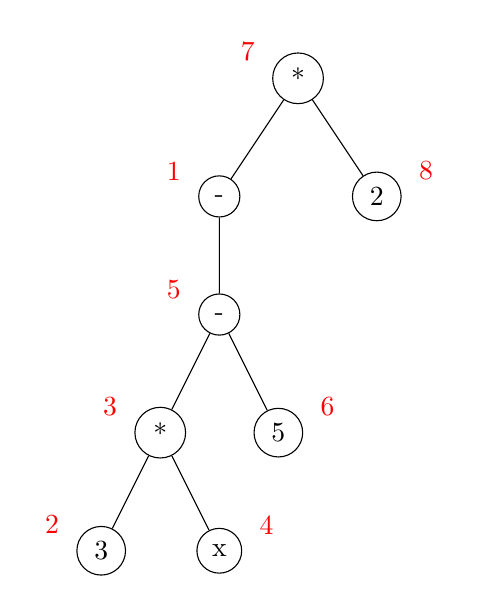
\begin{tikzpicture}[
      level distance=1.5cm,
      level 1/.style={sibling distance=2cm},
      level 2/.style={sibling distance=2cm},
      level 3/.style={sibling distance=1.5cm},
      every node/.style={draw, circle, align=center},
    ]
      \node[label={[label distance=0.1cm, text=red]165:7}] {*}
        child {
          node[label={[label distance=0.1cm, text=red]165:1}] {-}
          child {
            node[label={[label distance=0.1cm, text=red]165:5}] {-}
            child {
              node[label={[label distance=0.1cm, text=red]165:3}] {*}
              child {
                node[label={[label distance=0.1cm, text=red]165:2}] {3}
              }
              child {
                node[label={[label distance=0.1cm, text=red]15:4}] {x}
              }
            }
            child {
              node[label={[label distance=0.1cm, text=red]15:6}] {5}
            }
          }
        }
        child {
          node[label={[label distance=0.1cm, text=red]15:8}] {2}
        };
    \end{tikzpicture}
    \caption{\\Modificeret Inorder Travesal}
  \end{subfigure}
  \hfill
  \begin{subfigure}{0.3\textwidth}
    \centering
    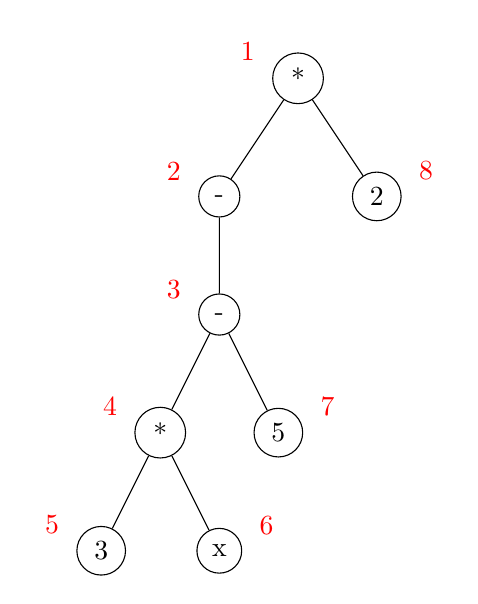
\begin{tikzpicture}[
      level distance=1.5cm,
      level 1/.style={sibling distance=2cm},
      level 2/.style={sibling distance=2cm},
      level 3/.style={sibling distance=1.5cm},
      every node/.style={draw, circle, align=center},
    ]
      \node[label={[label distance=0.1cm, text=red]165:1}] {*}
        child {
          node[label={[label distance=0.1cm, text=red]165:2}] {-}
          child {
            node[label={[label distance=0.1cm, text=red]165:3}] {-}
            child {
              node[label={[label distance=0.1cm, text=red]165:4}] {*}
              child {
                node[label={[label distance=0.1cm, text=red]165:5}] {3}
              }
              child {
                node[label={[label distance=0.1cm, text=red]15:6}] {x}
              }
            }
            child {
              node[label={[label distance=0.1cm, text=red]15:7}] {5}
            }
          }
        }
        child {
          node[label={[label distance=0.1cm, text=red]15:8}] {2}
        };
    \end{tikzpicture}
    \caption{\\Preorder Traversal}
  \end{subfigure}
  \hfill
  \begin{subfigure}{0.3\textwidth}
    \centering
    \begin{tikzpicture}[
      level distance=1.5cm,
      level 1/.style={sibling distance=2cm},
      level 2/.style={sibling distance=2cm},
      level 3/.style={sibling distance=1.5cm},
      every node/.style={draw, circle, align=center},
    ]
      \node[label={[label distance=0.1cm, text=red]165:8}] {*}
        child {
          node[label={[label distance=0.1cm, text=red]165:6}] {-}
          child {
            node[label={[label distance=0.1cm, text=red]165:5}] {-}
            child {
              node[label={[label distance=0.1cm, text=red]165:3}] {*}
              child {
                node[label={[label distance=0.1cm, text=red]165:1}] {3}
              }
              child {
                node[label={[label distance=0.1cm, text=red]15:2}] {x}
              }
            }
            child {
              node[label={[label distance=0.1cm, text=red]15:4}] {5}
            }
          }
        }
        child {
          node[label={[label distance=0.1cm, text=red]15:7}] {2}
        };
    \end{tikzpicture}
    \caption{\\Postorder Traversal}
  \end{subfigure}
  \begin{align*}
      \text{Modificeret Inorder Traversal:} \quad & - (3 \cdot x - 5) \cdot 2 \\
      \text{Preorder Traversal:} \quad &  \cdot - - \cdot 3\, x\, 5\, 2  \\
      \text{Postorder Traversal:} \quad & 3\, x\, \cdot 5\, - -  2\, \cdot
  \end{align*}
  \caption{Træet fra \ref{fig:expression_tree} med forskellige travesal metoder}
  \label{fig:expression_tree_traversal}
\end{figure}


Vi vil i \ref{sec:expression_module} betragte hvordan vi kan implementere et mondul som kan repræsentere ligningsudtryk ved brug af prefix notation.
Postorder Traversal blive anvendt til at kunne rekursivt simplificere og evaluere ligningsudtryk.

Grundet præcedens regler i infix notation, er det nødvendigt at modificere Inorder Traversal, da unære noder altid skal håndteres før dens børn. Desuden vil det også være nødvendigt at implementere regler for at håndtere parenteser, hvis der ønskes en symbolsk ligning. Den modificeret Inorder Traversal anvendes til at kunne visualisere ligningsudtryk i infix notation.


\subsubsection{Ligningsudtryk mondulet} \label{sec:expression_module}
Efter at have lavet et mondul til at repræsentere tal mængder, er det nu muligt at kunne implementere et mondul som kan repræsentere ligningsudtryk. Vi begynder ved at definere en polymorf type for et ligningsudtryk \ref{expr_type}. Typen består af en række konstruktører, som repræsentere de matematiske operationer vi ønsker at kunne anvende, samt en konstruktør N for at repræsentere matematiske strukturer og X for at repræsentere variable. Vi begynder med at betragte matematiske strukturer, i form af de tal mængder vi har definerede som Number \ref{number_type}. Vi vil senere betragte hvordan det vil være muligt at udvide programmet til at kunne repræsentere flere matematiske strukturer så som vektorer.     

\begin{lstlisting}[
    language={FSharp}, 
    label={expr_type}, 
    caption={Typen for Expr}
    ]
type Expr<'a> = 
    | X of char
    | N of 'a
    | Neg of Expr<'a>
    | Add of Expr<'a> * Expr<'a>
    | Sub of Expr<'a> * Expr<'a>
    | Mul of Expr<'a> * Expr<'a>
    | Div of Expr<'a> * Expr<'a>
\end{lstlisting}

Expr\textless'a\textgreater{}  typen er dermed en polymorf type, hvor 'a er typen for den matematiske struktur hvor vi kan lave brugerdefinerede matematiske operationer. Et exemplar på en Expr\textless Number\textgreater{}  er givet i \ref{lst:expr_example}. 

\begin{lstlisting}[style=output, label={lst:expr_example}, caption={$-(3 \cdot x - 5) \cdot 2$ som et udtryks træ. Funktionen tree bliver beskrevet i \ref{sec:expression_generation}.}]
> tree "-(3*x-5)*2";;
val it: Expr<Number> = 
  Mul (Neg (Sub (Mul (N (Int 3), X 'x'), N (Int 5))), N (Int 2))
\end{lstlisting}

Signatur filen indeholder overloadings på de matematiske operationer, så de kan anvendes mellem ligningsudtryk. Samt en funktion \textcolor{red}{eval} til at evaluere et ligningsudtryk. 
\lstinputlisting[
    language=FSharp,
    label={Number_fsi},
    caption={Signatur filen for Expression mondulet}
    ]{../modules/Expression.fsi}



De overloadede matematiske operatorer i Expressions, laver overflade evalueringer samt simplifikationer på deres respektive argumenter. Overfalde evalueing vil sige at de individuellen funktioner kun betragter de to øverste niveauer på de lignings udtryk træer de tager som input, mullige implementeringer af addition og multiplikation er givet i \ref{lst:mul_expr}. 

\begin{lstlisting}[
  language={FSharp}, 
  label={lst:mul_expr}, 
  caption={Addition og multiplikation af to ligningsudtryk}
  ]
// add: Expr<Number> -> Expr<Number> -> Expr<Number>
let rec add e1 e2:Expr<Number>  =
  match e1, e2 with
  | N a, N b                            -> N (a + b)
  | N a, b | b, N a when isZero a       -> b
  | Mul(a, X b), Mul(c, X d) 
  | Mul(X b, a), Mul(c, X d)
  | Mul(a, X b), Mul(X d, c) 
  | Mul(X b, a), Mul(X d, c) when b = d -> Mul(add a c, X b)  
  | _, _                                -> Add(e1, e2)

// mul: Expr<Number> -> Expr<Number> -> Expr<Number>
let mul e1 e2:Expr<Number> =
  match e1, e2 with
  |N a, N b                       -> N (a * b)
  |N a, b | b, N a when isOne a   -> b
  |N a, _ | _, N a when isZero a  -> N zero
  | _, _                          -> Mul(e1, e2)
\end{lstlisting}


\subsubsection{Generering af Ligningsudtryk}\label{sec:expression_generation}
% KAN lave PBT
    
\subsection{Evaluering af ligningsudtryk}
\subsubsection{PBT af evalueringen} % #TODO
\subsection{Simplifikation af Ligningsudtryk} \label{sec:simplification_expression}
\subsubsection{PBT af simplifikationen} % Beskriv hvordan man laver property based testen før simplifikationen

\subsection{differentiering af Ligningsudtryk}
    

\end{document}

